\section{Building Thom spaces} % <<<
\label{BuildingThomSpaces}
\ifx\OutputBuildingThomSpaces\undefined\else
We'll now start attacking the second part of the vector field problem.  Recall that the Stiefel manifold $V_{n, k}$ of $k$-frames on $\Rbb^n$ is given by $(n \times k)$-matrices with orthonormal columns, and projection onto the first column gives a fiber bundle $V_{n, k-1} \into V_{n, k} \onto S^{n-1}$.  The existence of a section $s$ of this bundle is equivalent to the existence of $(k-1)$ orthonormal vector fields on $S^{n-1}$.

Now we will find a consequence for the existence of such a section in the homotopy theory of $\RP^{k-1}$.  To start with, there are two important facts about $\RP^{k-1}$.  The first is the existence of a fiber bundle $\Zbb_2 \into S^{k-1} \onto \RP^{k-1}$ obtained by identifying antipodal points on $S^{k-1}$.  The second is the existence of the ``tautological line bundle'' $L = \{(l, x) \in \RP^{k-1} \times \Rbb^k \mid x \in l\} \onto \RP^{k-1}$, where one thinks of $\RP^{k-1}$ as the space of lines through the origin on $\Rbb^k$.  These two constructions are, of course, related: there is a metric on $L$ induced by the metric in $\Rbb^k$; taking the vectors of length $1$ in each fiber gives $S(L)$, the unit sphere bundle of $L$, and $S(L) \cong S^{k-1}$.

On the other hand, we can recover $L$ as $S^{k-1} \times_{\Zbb_2} \Rbb$; this is an example of the ``Borel construction.'' % define what a twisted product is.  it would a lso be useful to talk about why the Borel construction is useful; you can sort of always move to your favorite spot in the fiber.  this definition should also match use of the borel construction in lecture 6
More generally, if $F$ is any space with a $\Zbb_2$ action, we get a bundle with fiber $F$ by taking $F \into S^{k-1} \times_{\Zbb_2} F \onto \RP^{k-1}$.  What follows from a section $s$ of $V_{n, k} \onto S^{n-1}$ is:
\begin{lem}
If there is a section $s$, then there is a bundle map $\shat$ over $\RP^{k-1}$ of the form
\begin{ctikzcd}
\edgellap{\RP^{k-1}\times S^{n-1}=}S(n\epsilon) \rar["\shat"]\dar & S(nL) \edgerlap{{}=S^{k-1}\times_{\Zbb/2}S^{n-1}}\dar\\
 \RP^{k-1} \rar[equal]& \RP^{k-1}
\end{ctikzcd}
which acts as the identity on the fiber over the point $\pm e_1$, which we take as the basepoint in $\RP^{k-1}$.
(Here $\epsilon$ is the trivial bundle of dimension $1$ and $\Zbb$ acts on bundles by direct sum.)
\end{lem}
\begin{proof}
Define $\shat: \Rbb^k \times S^{n-1} \to \Rbb^k \times S^{n-1}$ by $\shat(x, v) = (x, s(v) x)$.  It is straightforward to see $|s(v) x| = 1$ if $|x| = 1$, so $\shat$ maps $S^{k-1} \times S^{n-1} \to S^{k-1} \times S^{n-1}$.  Quotienting the target by $\Zbb_2$, we have \[\shat(-x, v) = (-x, -s(v)x) = (x, s(v) x) = \shat(x, v),\] so it descends to a quotient on the source: $\shat: \RP^{k-1} \times S^{n-1} = S(n \epsilon) \to S^{k-1} \times_{\Zbb_2} S^{n-1} = S(nL)$.  Finally, $s(v)e_1 = v$ (as $s$ is a section), so $\shat(e_1, v) = (e_1, v)$.
\end{proof}
One point worth mentioning here is that $\shat$ could have been defined as a map $n \epsilon \to n L$, but it would not necessarily have been linear on each fiber (as $s(v)$ is not necessarily linear), so the map would not have been in a strict sense a map of vector bundles.  Previously, we constructed such sections $s$ using Clifford algebras, and in that case $s$ was in fact linear.  In some sense, then, the problem is to find out whether you can get more vector fields by modifying them in some clever way.

The fact that $\shat$ induces the identity over $\pm e_1$ means that $\shat$ induces a homotopy equivalence on each fiber.  Explicitly, for any open and connected $U \subseteq \RP^{k-1}$ such that $nL|_U$ is trivial and such that $\shat_b$ is a homotopy equivalence for some $b \in U$, it follows that $\shat$ induces a map $U \to \Hom(S^{n-1}, S^{n-1})$.  As $U$ is connected, it lands entirely in one path-connected component of $\Hom(S^{n-1}, S^{n-1})$, and hence the map on fibers is a homotopy equivalence.

We have two bundles $E$ and $E'$ over a base $B$ and a bundle map $f: E \to E'$ which induces a homotopy equivalence on each fiber.  What we really want is a map $g$ going back so that $fg$ and $gf$ are homotopic through bundle maps to the respective identity maps;  $f$ is then called a ``fiber homotopy equivalence.''  Fortunately there is a very nice theorem due to Dold:
\begin{thm}[Dold]\label{LemmaOfDold}
Suppose $E$ and $E'$ are fibrations over $B$ with a bundle map $f$ inducing a homotopy equivalence on each fiber.  If $E$ and $E'$ have the homotopy type of CW complexes and $B$ is connected, then $f$ has a fiber homotopy inverse.
\end{thm}
\begin{proof}
See \cite{James}.
\end{proof}
In this context, the lemma gives
\begin{cor}
If $V_{n, k} \onto S^{n-1}$ sections, then $S(nL) \onto \RP^{k-1}$ is fiber homotopy trivial.
\end{cor}
Ultimately we will show the result of Adams that this implies that $k \le \rho(n) - 1$, i.e., that $a_k$ divides $n$.


\begin{wrapfigure}{r}{0.3\textwidth}
\centering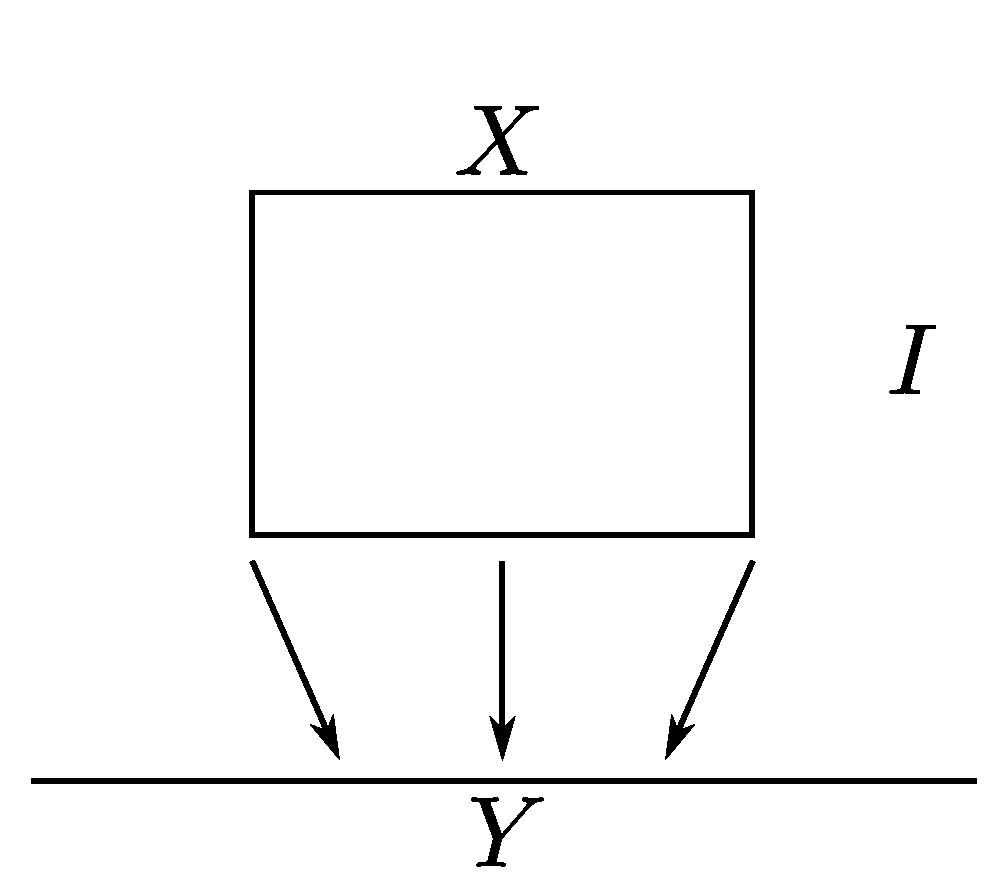
\includegraphics[width=0.2\textwidth]{figures/fig7.pdf}
\caption{\small Diagram of the mapping cylinder of $f$.}
\end{wrapfigure} % define the mapping cylinder, since we defined the mapping cone earlier.  in fact, this figure belongs to such a discussion, and should be treated separately.  why is this important that we can do it for "any" sphere bundle??
Next we look at the consequences of the discussion so far in terms of Thom spaces.  Suppose $E \onto B$ is a vector bundle with a metric, so there's a nice sphere bundle $p$ defined as the composite $S(E) \into E \onto B$.  In order to understand the map $p$, we could look again at the mapping cone $Cp = B \cup_p C_{S(E)}$ of $p$.

Given a map $f:X\to Y$, we can construct the cone $Cf$ in two stages, leaving pinching the cone for the ``second stage''. The intermediate space $Mf=X\times I\cup_f Y$ is called the ``mapping cylinder,'' and it is homotopy equivalent to $Y$.  Moreover there is a nice inclusion $X \into Mf$ which is a cofibration. Then $Cf$ is obtained by collapsing the image of $X$ in $Mf$.

In fact, it doesn't matter how you replace the space $Y$ with a homotopy equivalent space: as long as the map $f$ is replaced by a cofibration, collapsing out its image we obtain a space homotopic to the mapping cone.
%This is true, right?

Now in the case of $p: S(E) \onto B$, the mapping cone is called the Thom space, $T(E)$.
One can think of the mapping cylinder $p:S(E)\to B$ as being the disk bundle $D(E)$ of vectors of length less than or equal to $1$; the Thom space is then the quotient space $D(E) / S(E)$.

As a passing (but important) remark, the fibers of these two bundles over a basepoint $b \in B$ are $S^{n-1} \subset S(E)$ and $D^n \subset D(E)$, and pinching the former out of the latter gives an $S^n$ in $T(E)$.  So if $B$ is connected and $E$ is oriented, the Thom space comes with a unique, distinguished class in $\pi_n T(E)$.

\begin{wrapfigure}{r}{0.5\textwidth}
\centering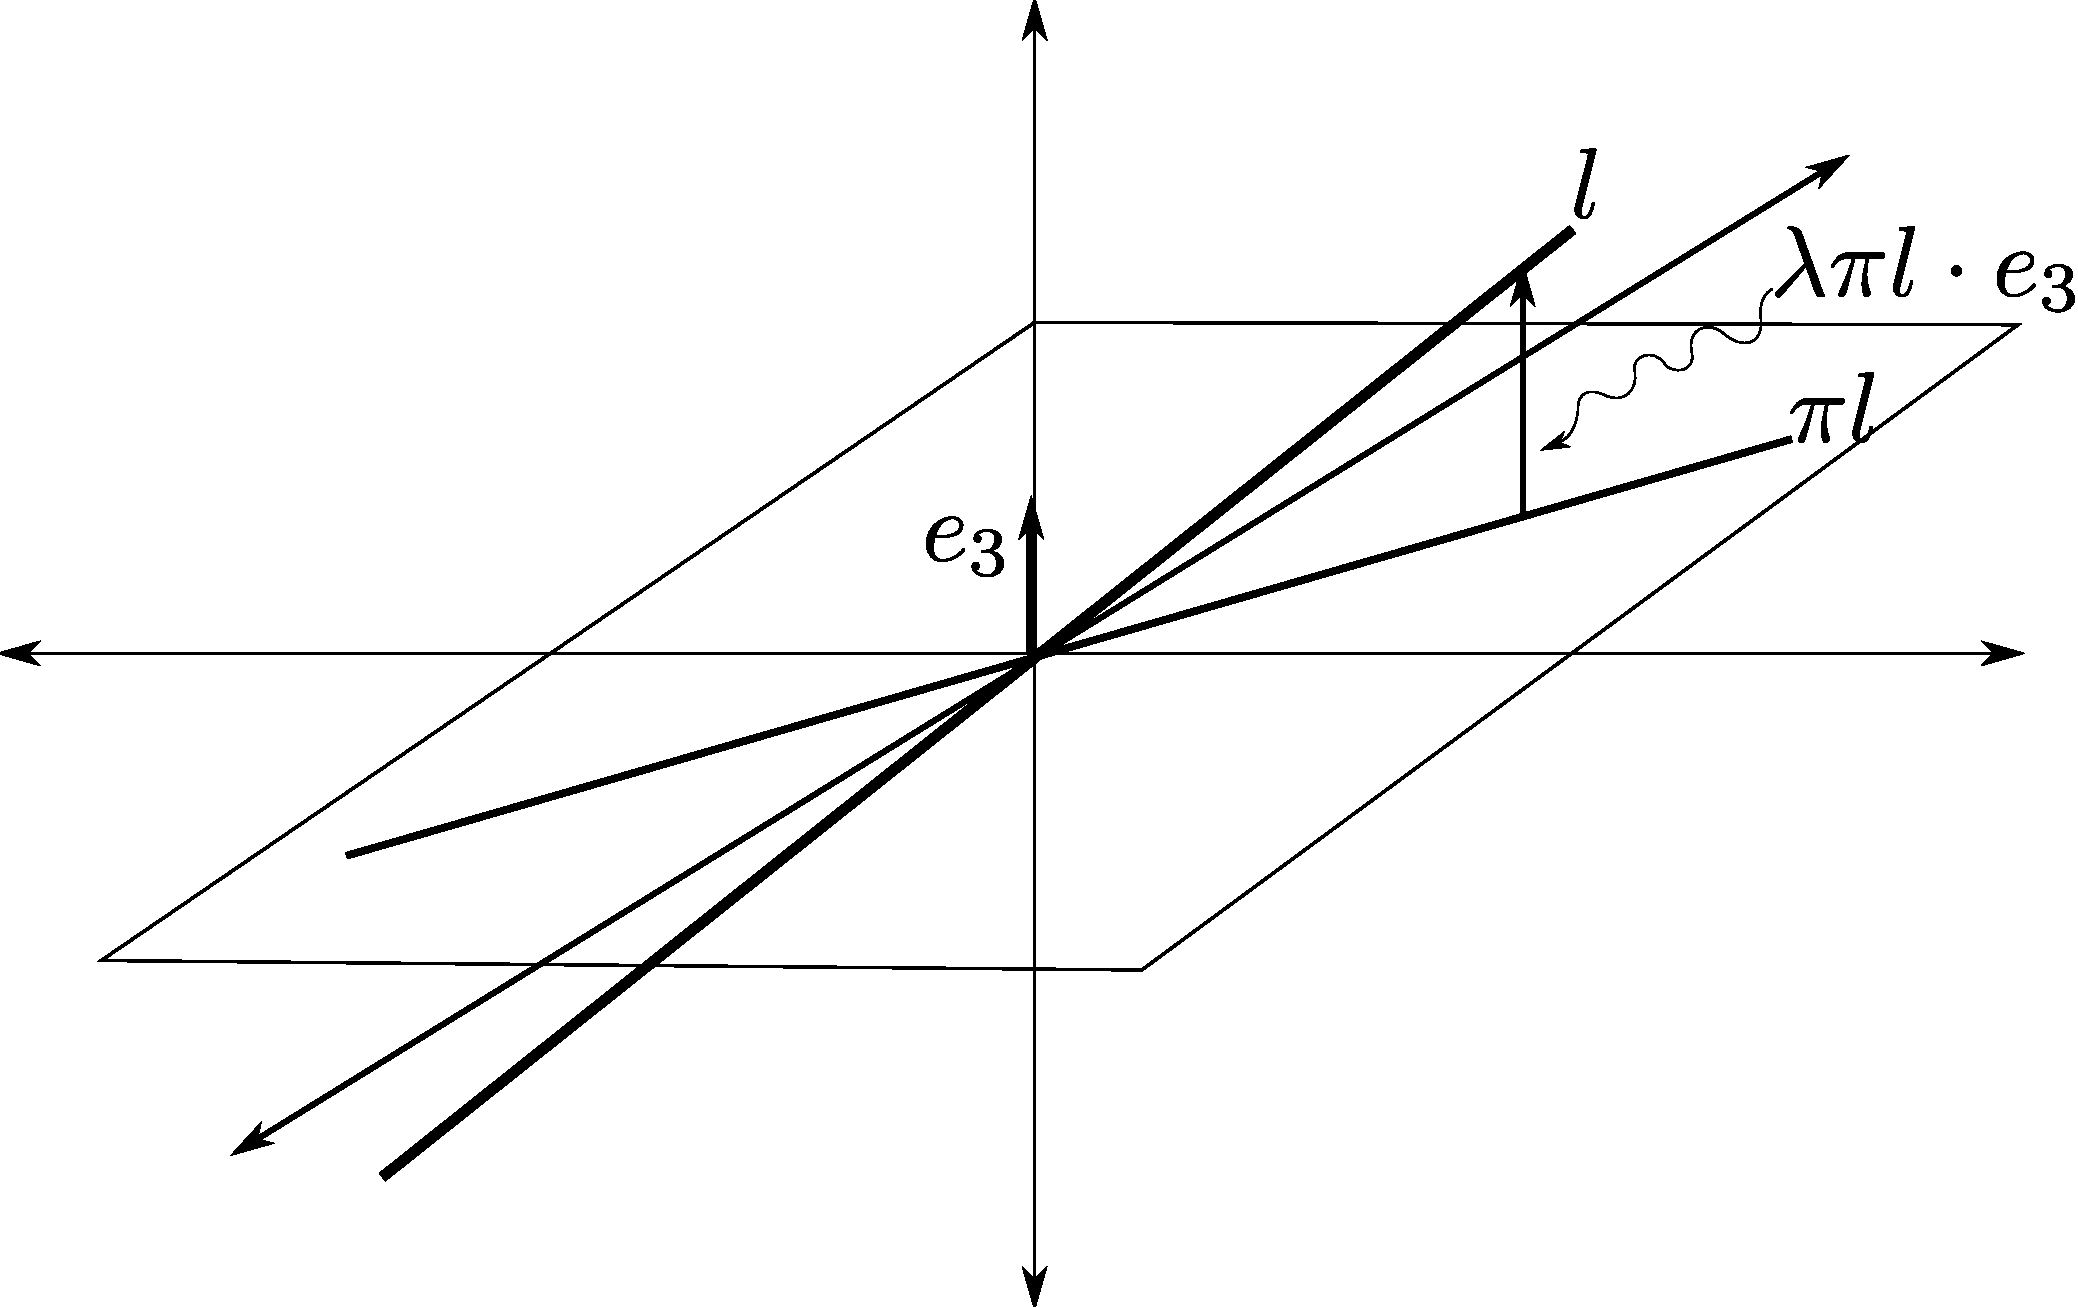
\includegraphics[width=0.4\textwidth]{figures/fig8.pdf}
\caption{\small Recovering $l$.}
\end{wrapfigure} % how can we make it clear that the lambda_i depend upon the point l in RP^k-1?
Next, we return to $nL$, the bundle over $\RP^{k-1}$, where $L$ is the tautological line bundle.  We claim that this bundle is the normal bundle $\nu$ of the inclusion $\RP^{k-1} \into \RP^{n+k-1}$ induced by the inclusion $\Rbb^k \into \Rbb^{n+k}$.  To wit, pick a point $l \in \RP^{n+k-1}$ parametrized as $l(t)$, a line in $\Rbb^{n+k}$.  Let $\pi l \in \RP^{k-1}$ be the projection of this line to a line in $\Rbb^k$.  We can recover the line $l$ in $\Rbb^{k+n} \cong \Rbb^k \times \Rbb \times \cdots \times \Rbb$ by $l(t) = (\pi l(t), \lambda_1(\pi l(t)), \ldots, \lambda_n(\pi l(t)))$ for some functions $\lambda_i$ dependent upon $l$.  Clearly $\lambda_i(rv) = r \lambda_i(v)$, so $\lambda_i \in L^*$.  Hence the normal bundle can be identified with $nL^*$.  Since $nL$ comes equipped with a metric, this gives an isomorphism of the normal bundle $\nu$ with $nL$.

% what?
But there's even more structure around.  \ConfusedBox{ Remarking that $\RP^{n+k-1}$ forms a vector bundle of rank $n$ over $\RP^{k-1}$ and using the inclusion of the open unit ball in $\Rbb^n$ to $\Rbb^n$, \textsc{(what does this mean?)}} one can construct a map from $D(\nu)$ to $\RP^{n+k-1}$ such that $S(\nu)$ maps to $\RP^{n-1}$ and which is a relative homeomorphism $(D(\nu), S(\nu)) \to (\RP^{n+k-1}, \RP^{n-1})$.\footnote{One candidate for the map $D(\nu)\to\RP^{n+k-1}$ can be specified as follows. View $D(\nu)$ as $D(nL)$, where $nL\subset \RP^{k-1}\times (\Rbb^k)^n$ inherits its metric from the standard Euclidean metric on $(\Rbb^k)^n$. Then a point of $D(\nu)$ is an $n+1$-tuple $(\Rbb\{z\},r_1z,r_2z,\ldots,r_nz)$, where $z\in R^k$ has length one, $\|r\|^2=\sum r_i^2\leq1$. The map sends this point to $(z,r_1,r_2,\ldots,r_n)$.}
It follows that the Thom space of $nL$ is $T(nL)\simeq\RP^{n+k-1}/\RP^{n-1}$. In particular, if $nL$ is being fiber homotopy trivial, then $T(n\epsilon) \simeq T(nL) \cong \RP^{n+k-1}/\RP^{n-1}$.
%
% sends $([z], r_1z, \ldots, r_nz)\in D(\nu)\subseteq \Rbb P^{k-1}\times (\Rbb^k)^n$, where $[z]=\Rbb z\in\RP^{k-1}$ for $z\in\Rbb^k$ to }

% >>>
\fi
\BoxedNote{
%\Bullet Lemma of Dold: if a map of fibrations (with the homotopy type of CW-complexes) over a connected base $B$ is a homotopy equivalence on each fiber, it has a fiber homotopy inverse.
%
%\Bullet Lemma of Dold: maps of nice fibrations over the same connected base restricting to a homotopy equivalence on each fiber have fiber homotopy inverses.
%
\Bullet Dold: suppose $f:E_1\to E_2$ is a map of fibrations $E_i\downarrow B$, the $E_i$ have the homotopy type of a CW-complex, and $B$ is connected. Then if $f$ restricts to a homotopy equivalence on each fiber, it has a fiber homotopy inverse.

\Bullet $nL\onto \Rbb P^{k-1}$ is the normal bundle of the inclusion into $\Rbb P^{n+k-1}$.

\Bullet If $V_{n, k} \onto S^{n-1}$ sections, then $S(nL)\onto \Rbb P^{k-1}$ is fiber homotopy trivial.

\Bullet $T(nL)\simeq \RP^{n+k-1}_n:=\Rbb P^{n+k-1}/\Rbb P^{n-1}$ ``stunted projective space'' (any $n,k$).

\Bullet In particular, if $S^{n-1}$ admits $k-1$ vector fields, $T(n\epsilon)\simeq T(nL)\simeq \Rbb P^{n+k-1}_n$.
}
\section{Facts about Thom spaces} % <<<
\label{FactsAboutThomSpaces}
\ifx\OutputFactsAboutThomSpaces\undefined\else
We'll now look at Thom spaces in more detail, and in particular in relation to some other standard constructions on fiber bundles.  First of all, we have a product: given two bundles $F \to E \to B$ and $F' \to E' \to B'$, we can build a bundle $F \times F' \to E \times E' \to B \times B'$.  Now if $B = B'$, you can pull this bundle back along the diagonal map to a bundle $F \times F' \to E \times_B E' \to B$, called the ``fiberwise product.''  If $E$ and $E'$ are vector bundles, then $E \times_B E'$ is called the ``Whitney sum,'' denoted $E \oplus E'$.

\begin{wrapfigure}{r}{0.33\textwidth} % maybe it would be better to give a drawing more reflective of the construction
\centering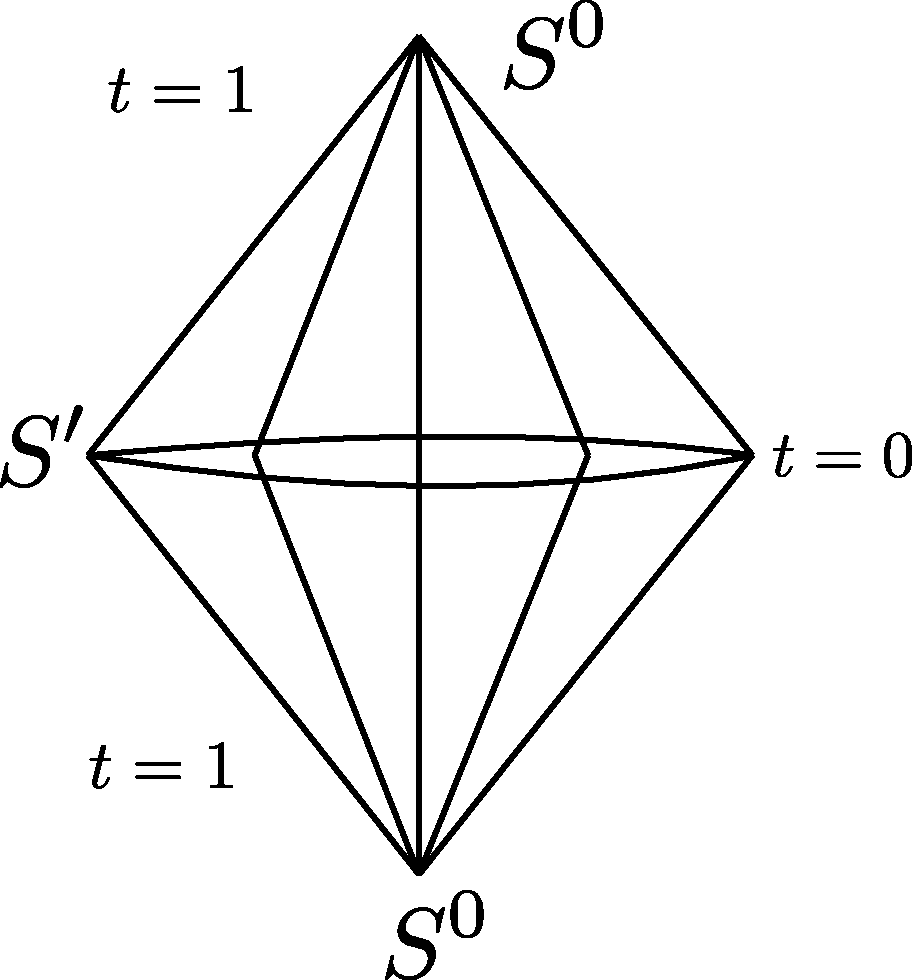
\includegraphics[width=0.3\textwidth]{figures/fig9.pdf}
\caption{\small A diagram of $S^0 \ast S^1$.}
\end{wrapfigure}
If $E$ and $E'$ are sphere bundles, this construction isn't very satisfying, because a sphere cross a sphere isn't another sphere.  However, the join of two spheres is another sphere.  Here's another way of looking at the join\footnote{As an aside, we define $X \ast \emptyset = \emptyset \ast X = X$.} (we will return to the join often, and try as often as possible to give different definitions of it!):
\[
X \ast Y = \frac{X \times I \times Y}{(x, 1, y) \sim (x, 1, y'), (x, 0, y) \sim (x', 0, y)}.
\]
Now we define a fiberwise join by doing this on each fiber to get a bundle $F \ast F' \to E\mathop{\widehat\ast}E' \to B \times B'$, where \[E\mathop{\widehat\ast}E' = \frac{E \times I \times E'}{\substack{\hbox{$(x, 1, y) \sim (x, 1, y')$ if $p'y = p'y'$}, \\ \hbox{$(x, 0, y) \sim (x', 0, y)$ if $px = px'$.}}}\]  One can check that this construction yields something locally trivial.  The fiberwise join for sphere bundles is related to the fiberwise product of vector bundles: if $V$ and $W$ are vector bundles, then $S(V \times W) = SV \,\widehat \ast \,SW$.  Moreover, if $B = B'$ we can once again pull back by the diagonal map on $B$, and we get $SV \ast_B SW = S(V \oplus W)$.

In the case that $Y = \ptspace$, $X \ast Y = CX$ is the cone over $X$.  Applying this in the fiberwise join, we transport a bundle $F \to E \to B$ to a bundle $CF \to C_B E \to B$, where $C_BE:=E\mathop{\widehat\ast}B$.  Applying this to a sphere bundle $E \to B$ gives a disk bundle $C_B E \to B$, and it's easy to check that if $V$ is a vector bundle, then $D(V) = C_B S(V)$, so we have a way of recovering the disk bundle from the sphere bundle.

Now back to Thom spaces.  Recall that if $E \onto B$ is a sphere bundle, its Thom space is $T(E) = C_B E / E$, and if the fiber over the basepoint of $B$ in $E$ is $S^{n-1}$, then $CS^{n-1} = D^n \subset C_B E$, which becomes an $S^n \subset T(E)$.  The Thom space comes equipped with a canonical basepoint which is the image of $E$, which has been crushed to a point.  If $V \onto B$ is a vector bundle, then $T(V)$ is defined to be $T(S(V))$, and also $T(0) = \pt{B}:=B \amalg \ptspace$.\footnote{By convention, $0$ denotes the rank zero vector bundle.  In this case $S(0) = E = \emptyset$, and we write $T(\emptyset) = B / \emptyset = B \amalg \ptspace$ also by convention.  This is done so that the smash product identity below works.}

To understand this better, let's look at the trivial sphere bundle $B \times S^{n-1} \to B$.  Here, we have $T(B \times S^{n-1}) = B \times D^n / B \times S^{n-1}$.  Now as $S^n\cong D^n/S^{n-1}$, it follows that:
\[T(B \times S^{n-1}) = \frac{B \times D^n}{B \times S^{n-1}} \cong \frac{B \times S^n}{B \times \ptspace} \cong \pt{B} \sprod S^n = \Suspend^n(\pt{B}),\]
and so the Thom space of a bundle can be thought of as a twisted sort of suspension.

Here's an important fact: $T(E\, \widehat \ast\, E') = T(E) \sprod T(E')$, where $\sprod$ is the smash product of pointed spaces.  A rough proof in the special case that $E = SV$ and $E' = SW$ for vector bundles $V\downarrow B$ and $V'\downarrow B'$ is:
%\begin{align*}
%TV \sprod TW & = T(S(V)) \sprod T(S(W)) \\ %A bit wordy
%& = \frac{DV}{SV} \sprod \frac{DW}{SW} \\
%& = \frac{\frac{DV}{SV} \times \frac{DW}{SW}}{\frac{DV}{SV} \wsum \frac{DW}{SW}} \\
%& = \frac{DV \times DW}{(SV \times DW) \cup (DV \times SW)} \\
%& \cong \frac{D(V \times W)}{S(V \times W)} \\
%& = T(S(V \times W)) = T(E\,\widehat \ast\, E').
%\end{align*}
\[TV \sprod TW = \frac{DV \times DW}{(SV \times DW) \cup (DV \times SW)}\cong \frac{D(V \times W)}{S(V \times W)}= T(S(V \times W)) = T(E\,\widehat \ast\, E').\]
In the special case that $E' \to B'$ is $\Rbb^n \to \ptspace$, we get that $T(V \oplus n \epsilon) = T(V) \sprod S^n = \Suspend^n T(V)$.

Note that if $V$, $W$ are vector bundles over $B$, it is \textbf{not} the case that $T(V\oplus W)=T(V)\wedge T(W)$. However, we have a pullback diagram (drawn on the left) which induces a map of Thom spaces (drawn on the right). This map commutes with the inclusion of the copies of $S^{n+m}$ (where $\dim_*V=n$ and $\dim_*W=m$):
%
\begin{cjointikzcd}
\diagram
    V\oplus W \rar\dar & V\times W\dar  \\
    B \rar["\Delta"]   & B\times B
%
\diagram
 T((V\oplus W)\downarrow B) \rar& T((V\times W)\downarrow(B\times B) \rar[equal] & T((V\downarrow B)\wedge T(W\downarrow B))\\
                                & S^{n+m}    \ular\uar               \rar[equal] & S^n\wedge S^m\uar
\end{cjointikzcd}

The Thom space is useful for deciding whether a fiber bundle is trivial.  To this end, we observe that if $E$ and $E'$ are fiber homotopy equivalent $S^{n-1}$-bundles, then $T(E) \simeq T(E')$ relative to the copies of $S^n$ over the basepoint in $B$.
\begin{lem}\label{LemOnFHTrivialisations}
Suppose that $E \to B$ is an $S^{n-1}$-bundle. Then fiber homotopy equivalences $h:E\to B\times S^{n-1}$ are in bijection with maps $f:E\to S^{n-1}$ whose restriction to each fiber is a homotopy equivalence. Moreover, if any such maps exist (i.e.\ if $E\to B$ is fiber homotopy trivial), then each map $f$ induces a ``coreduction'':
%
\begin{ctikzcd}
T(E) \rar & S^n\\
S^n\uar \urar["\simeq"']
\end{ctikzcd}
\end{lem}
%
%
\begin{proof}
Write $\pi_2:B\times S^{n-1}\to S^{n-1}$ for the second projection. Then (by the universal property of the product), fiber maps $h:E\to B\times S^{n-1}$ are in bijective correspondence with maps $f:E\to S^{n-1}$, via $h\mapsto \pi_2h$. Now we note that fiber homotopy equivalences $h$ correspond exactly to maps $f$ inducing a homotopy equivalence on each fiber. If such a map $f$ exists, it can be thought of as a bundle map
%
\begin{cjointikzcd}[intertext,row sep = tiny]
\diagram
    E \rar["f"]\dar & S^{n-1}\dar \\
    B \rar & \ast
%
\diagram \intertext{which induces a map on Thom spaces:}
%
\diagram
    T(E)\rar & S^n\edgerlap{=T(S^{n-1}\downarrow*)}\\
    S^n\ar[u]\ar[ur,"\simeq"']
\end{cjointikzcd}
%
and the homotopy equivalence of $f$ restricted to each fiber implies that the map $S^n\to S^n$ is a homotopy equivalence.
\end{proof}
\noindent Now the game is to find obstructions to the splitting off of this $n$-sphere, which is in fact the bottom-dimensional cell in $T(E)$.

Of course, what we really want is an obstruction to a fiber homotopy equivalence between $nL$ and $n \epsilon$, and a coreduction of $T(E)$ need not imply that $E$ itself is fiber homotopy trivial.  To find out what we \emph{do} get from a coreduction of $T(E)$, we look at another construction of the Thom space (and think of the name Bott when thinking about $T(E)$ in this way).  We build $T(E)$ in two steps:
\begin{enumerate}
\item Collapse to a sphere in each fiber $F$, i.e., take $D(F) / S(F)$ in each fiber of $E \to B$.  This gives a sphere bundle, along with a ``section at $\infty$'' given by the image of $S(F)$ in each fiber.
\item Collapse the section at $\infty$ to a point.
\end{enumerate}
This exhibits $T(E)$ as the sphere bundle $S(E \oplus \epsilon)$ with the $1$-section of $\epsilon$, which is homeomorphic to $B$, smashed to a point, so $T(E) = S(E \oplus \epsilon) / B$, after identifying $B$ with that section. % the difference here is that you're adding a point at infinity to each fiber, then collecting all the points at infinity together.

Now the fiber in $S(E \oplus \epsilon)$ is the same as the $S^n$ sitting in $T(E)$, so with this construction a coreduction for $T(E)$ gives
\begin{ctikzcd}
& S^n \dlar\dar\drar["\simeq"] &\\
S(E\oplus\varepsilon) \rar & T(E)\rar & S^n
\end{ctikzcd}


If the base $B$ is connected, then from Dold's theorem (\ref{LemmaOfDold}) it follows that $E \oplus \epsilon$ is fiber homotopy trivial. % this sentence is completely vacuous when B is a CW-complex, so who cares about Dold's theorem
So a coreduction of $T(E)$ implies that $S(E \oplus \epsilon)$ is fiber homotopy trivial.

This is a process of stabilization: the lesson of this discussion is that we have to play back and forth with various processes of this kind: suspend the Thom space, sum in a trivial bundle, and so on.  These connections yield the natural role of $K$-theory. % maybe we could include a diagram exemplifying that the Thom space of eps (+) E is the same as the suspension of the Thom space of E
\fi
\BoxedNote{
\Bullet The fiberwise join of fiber bundles was constructed. Given $E\downarrow B$, performing the join with $B\downarrow B$ yields a bundle $C_BE$, the fiberwise cone. This recoves the disk bundle from a sphere bundle, and gives another definition of the Thom space of a sphere bundle $E$: $C_BE/E$.

\Bullet $T(E\, \widehat \ast\, E') = T(E) \sprod T(E')$ for bundles $E\downarrow B$ and $E'\downarrow B'$.

\Bullet $T(V\times W\downarrow B\times B')=T(V)\sprod T(W)$, where $V\times W$ is the exterior direct sum of vector bundles $V\downarrow B$ and $W\downarrow B'$.

\Bullet If $V,W$ are vector bundles over $B$, then $T(V\oplus W\downarrow B)\to T(V\times W\downarrow B\times B)$ is not a homotopy equivalence, but is compatible with the various inclusions of spheres over basepoints.

\Bullet If $E,E'$ are f.h.eq.\ $S^{n-1}$-bundles then $T(E)\simeq T(E')$ relative to the copies of $S^n$ over the basepoint.

\Bullet A fiber homotopy trivialisation of an $S^{n-1}$-bundle $E\downarrow B$ induces a \emph{coreduction}: maps $S^n\to T(E)\to S^n$ with composite $\simeq\textup{id}$, splitting off the bottom cell.

\Bullet If a coreduction of $T(E)$ exists then $S(E\oplus\epsilon)$ is fiber homotopy trivial.
}
% >>>
\section{Building \texorpdfstring{$K$}{K}-theory and \texorpdfstring{$J$}{J}-theory} % <<<
\label{BuildingKandJtheory}
\ifx\OutputBuildingKandJtheory\undefined\else
Now a few introductory words on $K$-theory: let $X$ be a pointed %finite complex (it is at least necessary that $X$ be a
compact Hausdorff space.  Let $\Vect(X)$ be the set of isomorphism classes of vector bundles over $X$.\footnote{Why is $\Vect(X)$ a set?}  The Whitney sum gives a monoid structure to $\Vect(X)$, with zero given by the $0$-dimensional vector bundle.  Now one applies the ``Grothendieck construction,'' which simply means to add formal inverses, making a group; explicitly, we form equivalence classes of pairs $(V,W)$ under the equivalence relation in which $(V, W) \sim (V', W')$ iff $E + V + W' \cong V' + W + E$ for some vector bundle $E$.  Here, $(V, W)$ is supposed to represent the formal difference ``$V - W$''.  This is an abelian group, called $KO(X)$.

Now it may not seem that $KO(X)$ has topological significance, but in view of the last lecture, it quickly becomes apparent that it does.  For if $V \oplus n\epsilon \cong W \oplus n\epsilon$ for some $n$ ($V$ and $W$ are said to be ``stably isomorphic''), then the classes $[V]$ and $[W]$ are equal in $KO(X)$.  Moreover, as $X$ is a compact Hausdorff space, it goes both ways.  Suppose $[V] = [W]$, so $V + E \cong W + E$ for some $E$.  Over a compact Hausdorff space, any vector bundle $E$ is a subbundle of a sufficiently big trivial bundle
\begin{ctikzcd}
E \rar[hook]\dar & X\times \Rbb^N\dlar\\
X
\end{ctikzcd}
as we shall soon see.  By choosing a metric on $\Rbb^N$, we get an orthogonal complement $F \to X$ such that $E \oplus F$ is trivial.  Then $V \oplus E \oplus F \cong W \oplus E \oplus F$, so $V$ and $W$ are stably isomorphic!

%Throughout, let $X$ be a pointed compact Hausdorff space.  Recall that $KO(X)$ was defined to be the abelian group given by the Grothendieck construction on the monoid $\Vect(X)$.
If $f: X \to Y$ is a map and $E \to Y$ is a vector bundle, then $E$ pulls back by $f$ to a vector bundle $f^* E \to X$, so we have a map $f^*: KO(Y) \to KO(X)$.  Pullbacks by homotopic maps induce isomorphic bundles, so $f \simeq g$ implies $f^* = g^*$.  Hence $KO$ is a contravariant functor $ \mathit{ho}\mathsf{Top} \to \mathsf{AbGrp}$. % it would be smart to come up with a notation for vector bundles, like f^* E downarrow X

Now the canonical maps $\ptspace \to X \to \ptspace$ induce maps $KO(\ptspace) \stackrel{\eta}{\to} KO(X) \stackrel{\epsilon} \to KO(\ptspace)$.  It is clear that $KO(\ptspace) = \Zbb$, that $\im \eta$ consists of trivial bundles, and that $\epsilon(V,W)=\dim_*(V)-\dim_*(W)$ takes the difference of the dimensions of the fibers over the basepoint.  Reduced $KO$-theory is defined in terms of these maps.  There are two equivalent definitions: % point out that this sequence is induced by the triangle pt --> X --> pt, with the composite a homotopy equivalence.
\[ % this isn't defined piecewise, so we are we using this bracket notation?
\widetilde{KO}(X) = \begin{cases}
\ker \epsilon & \hbox{: virtual vector bundles, i.e., formal differences $V - W$ with the same rank, or} \\
\coker \eta & \hbox{: i.e.,\ $\Vect(X)/\approx$, where $V\approx W$ iff $V \oplus m \epsilon \cong W \oplus n \epsilon$ for some $m,n\geq0$}.
%\coker \eta & \hbox{: $[V] = [W]$ if and only if $V \oplus m \epsilon \cong W \oplus n \epsilon$}. % aaron finds this line confusing, so we should change it
\end{cases}\]
The description here of $\coker\eta$ is correct as any equivalence class in $KO(X)$ contains a pair of the form $(V,n\epsilon)$. To obtain such a pair in the class of $(V',W')$, find $W''$ such that $W'+W''$ is trivial, as above, and then $(V',W')\sim (V'+W'',W'+W'')$.
Notice that $\coker\eta$ is the just the monoid $\Vect(X)$ taken modulo the equivalence relation generated by $V\approx V\oplus\epsilon$, which turns out to be a group, by the above argument.

Similarly, any equivalence class in $\ker\epsilon$ contains a pair of the form $(V,n\epsilon)$ where $n=\dim_*(V)$. We often denote this equivalence class $[V]-n$.


Next we'll see, as advertised, how to embed a vector bundle into a high-dimensional trivial bundle.  Suppose $p: E \to X$ is a rank $n$ vector bundle.  Because $X$ is compact Hausdorff, it has a finite open cover $U_1, \ldots, U_k$ that trivializes $E$.  That is, there are homeomorphisms $f_i$ with
\begin{ctikzcd}[column sep=small]
E|_{U_i}\drar["p"']\ar[rr,"f_i"] && U_i\times \Rbb^n \dlar["\pi"]\\
&U_i&
\end{ctikzcd}
such that the triangle commutes and $f_i$ is linear on each fiber.  Let $\phi_1, \ldots, \phi_k$ be a partition of unity subordinate to the cover $\{U_i\}$, and define maps $g_1, \ldots, g_k: E \to \Rbb^n$ by
\[
g_i =
\begin{cases}
E|_{U_i} \stackrel{f_i}{\to} U \times \Rbb^n \stackrel{(x, v) \mapsto \phi_i(x) \cdot v}{\longrightarrow} \Rbb^n, \\
\hbox{$0$ on $E$ away from $U_i$}.
\end{cases}\]
The $g_i$ give a linear embedding $f: E \to X \times (\Rbb^n)^k$ defined by $f(e) = (p(e), g_1(e), \ldots, g_k(e))$.

This map in fact gives more: to each $x \in X$ we associate the $n$-dimensional subspace $f(E_x)$ of $\Rbb^N$ with $N = nk$.  This induces a classifying map $h$ from $X$ to the Grassmannian of $n$-planes in $\Rbb^N$.  Over $G_{N, n}$ is the tautological $n$-plane bundle $E_{N, n}$, \[E_{N, n} = \{(v, p) \mid p \in G_{N, n}, \hbox{$v$ a member of the subspace associated to $p$}\}\] and we have in fact expressed $E \to X$ as the pullback of the tautological bundle along $h$.  From this point of view it is clear that the choice of $N$ is somewhat arbitrary; there are obvious inclusions $G_{N, n} \subseteq G_{N+1, n} \subseteq G_{N+2, n} \subseteq \cdots$, and $E$ can be induced from the tautological bundle over $G_{N, n}$ for any sufficiently large $N$.  Thus we have a classifying space $BO(n) = \bigcup_N G_{N, n}$, and it represents rank $n$ vector bundles over $X$ via $\Vect_n(X) \stackrel{\cong}{\to} [X, BO(n)]$.

What happens when we descend to $KO(X)$?  First, the equivalence $V \sim V \oplus \epsilon$ gives us $\widetilde{KO}$, % is Grothendieck(Vect) / this relation the same as Vect / this relation? Yes - Now discussed above.
so we get $\widetilde{KO}$ by identifying an element of $[X, BO(n)]$ with an element of $[X, BO(n+1)]$ when all it does is add a trivial bundle.  Now if $EO(n)$ is the tautological $n$-plane bundle over $BO(n)$, % should this be called the canonical O(n)-bundle?  should we warn the reader we're going to mix these things together using the Borel construction?
then $EO(n) \oplus \epsilon$ is an $(n+1)$-plane bundle, and there is a classifying map $BO(n)\to BO(n+1)$ for this bundle. We obtain a sequence:
\begin{ctikzcd}
\cdots \rar & BO(n) \rar & BO(n+1) \rar & \cdots
\end{ctikzcd}
of classifying maps whose colimit $\bigcup_n BO(n)$ is called $BO$, and $\widetilde{KO}(X) = [X, BO]$.\footnote{%
This argument can be summarised as follows: $\widetilde{KO}(X)=\textup{colim}[X,BO(n)]$, which equals $[X,\textup{colim}BO(n)]$ as $X$ is compact.
}
Finally, $KO$ remembers dimension, so $KO(X) = [X, \Zbb \times BO]$. % where Z keeps track of the virtual dimension

Now let's talk about $J$-theory.  If $V$ and $W$ are vector bundles over $X$, then we write $V \sim_J W$ if $S(V \oplus n \epsilon)$ and $S(W \oplus n \epsilon)$ are fiber homotopy equivalent for some $n\geq0$. This idea is analogous to $K$ on the level of sphere bundles, and defines an additive equivalence relation on $KO(X)$. $J(X)$ is defined to be the quotient of $KO(X)$ given by this relation, and $\widetilde J(X)$ the image of $\widetilde{KO}(X)$. % there should be an equation attached to this last sentence
Now from the Clifford algebra story we know that over $\RP^k$ the tautological line bundle $L$ has $a_k L \cong a_k \epsilon$. % this a_k was defined in day 2, remind the reader
Considering the class $[L] - 1 \in \widetilde{KO}(\RP^k)$, this means $a_k([L] - 1) = 0$. In fact: % say early on that we're going to identify n eps with n.
\begin{thm}[Adams]\label{AdamsKORPn}
$\widetilde{KO}(\RP^k)=\Zbb/a_k\Zbb$ generated by $[L]-1$.
$\widetilde{KO}(\RP^k) \stackrel{\cong}{\onto} \widetilde J(\RP^k)$ is an isomorphism.
\end{thm}
In other words, there are no other trivializations, and so % remind the reader that we were talking about coreductions earlier
\begin{cor}
If $S(nL) \to \RP^k$ is fiber homotopy trivial, then $a_k$ divides $n$. In particular, there are at most $\rho(n) - 1$ vector fields on $S^{n-1}$. % this should have a proof attached, reminding the reader of the chain of implications
\end{cor}
\begin{proof}
Suppose that $S(nL)$ is fiber homotopy trivial. Then $n[L]$ equals $n[\epsilon]$ in $\widetilde J(\Rbb P^k)$, and so $n([L]-1)=0$ in $\widetilde{KO}(\RP^k)$, implying that $a_k|n$. This demonstrates the first claim.

Now we saw in lecture \ref{CliffordAlgebras} that $a_k|n$ iff $k\leq \rho(n)-1$. We saw in lecture \ref{BuildingThomSpaces} that if $V_{n, k+1} \onto S^{n-1}$ sections, then $S(nL)\onto \Rbb P^{k}$ is fiber homotopy trivial. Thus, if $V_{n, k+1} \onto S^{n-1}$ sections, we must have $k\leq\rho(n)-1$.
\end{proof}
One of the things we get out of this theorem is that $\widetilde{KO}(\RP^k)$ is finite. In general: % really i think this and the previous immediate theorems should be moved down below Atiyah's theorem
\begin{thm}[Atiyah]
If $X$ is a finite connected complex, then $\widetilde J(X)$ is finite.
\end{thm}
\begin{proof}(Sketch, anyway.)
A vector bundle over $X$ is classified by a map $X \to BO(n)$.  Similarly a sphere bundle should have a similar classifying procedure.  In general, the structure group would have to be taken to be $\textup{Homeo}(S^{n-1})$, % use the same formula as below, but without the basepoints
but since we are only concerned with fiber homotopy equivalences we should be able to use the monoid $G_n$ of homotopy self-equivalences of $S^{n-1}$.  Such a classifying procedure exists; call the corresponding space $BG_n$.  Now there is a natural inclusion $O_n \into G_n$, and hence maps
\begin{ctikzcd}
BO(n)\rar \dar & BG_n\dar\\
BO \rar & BG
\end{ctikzcd}
We then make two claims: $\widetilde J(X)$ is the image of $[X, BO] \to [X, BG]$, and $[X, BG]$ is finite.  We prove this last part cell-by-cell, so what we really need to show is that $\pi_i(BG_n)$ is finite for $i$ much smaller than $n$.  Since $X$ is finite, $[X, BG] \simeq [X, BG_n]$ for some $n$ sufficiently larger than the top-dimensional cell of $X$, so this is enough.  There is a fibration $G_n \to EG_n \to BG_n$, and hence $\pi_i BG_n \cong \pi_{i-1} G_n$.  We are then left with showing that $\pi_i G_n$ is finite (again, for $i$ must smaller than $n$).  Now an element of $G_n$ is a map $S^{n-1} \to S^{n-1}$; by evaluating at the basepoint in $S^{n-1}$ we get a map $G_n \to S^{n-1}$.  This is a fibration whose fiber is homotopy equivalent to $\Loops^{n-1}_{\pm 1}S^{n-1} := \{f: (S^{n-1}, s_0) \to (S^{n-1}, s_0) : \deg f = \pm 1\} \subseteq \textup{Maps}(S^{n-1}, S^{n-1})$.  For $i$ much smaller than $n$, $\pi_i G_n \cong \pi_i(\Loops^{n-1}_\pm S^{n-1})$ and $\pi_i(\Loops^{n-1}_\pm S^{n-1}) \subset \pi_i(\Loops^{n-1} S^{n-1}) = \pi_{i+n-1} S^{n-1} = \Pi_i$, which is known to be finite by a theorem of Serre.
\end{proof}
\fi

\BoxedNote{
\Bullet For any bundle $E$ on a compact Hausdorff space there is a bundle $E'$ such that $E\oplus E'$ is trivial.

\Bullet$\widetilde {KO}(X)$ can be viewed as (i) $\Vect(X)/\approx$, where $\approx$ is generated by $V\approx X\oplus\epsilon$, or (ii) as equivalence classes of virtual vector bundles $V-W$, where $\dim V=\dim W$.

\Bullet Adams: $\widetilde{KO}(\RP^k)=\Zbb/a_k\Zbb$ generated by $[L]-1$, and the canonical epimorphism $\widetilde{KO}(\RP^k)\to\widetilde{J}(\RP^k)$ is an isomorphism, solving the vector field problem.

\Bullet Atiyah: $\widetilde J(X)$ is finite for $X$ a finite connected complex.
}

% >>>
